% This is samplepaper.tex, a sample chapter demonstrating the
% LLNCS macro package for Springer Computer Science proceedings;
% Version 2.20 of 2017/10/04
%
\documentclass[runningheads]{llncs}
%
\usepackage{graphicx}
% Used for displaying a sample figure. If possible, figure files should
% be included in EPS format.
%
% If you use the hyperref package, please uncomment the following line
% to display URLs in blue roman font according to Springer's eBook style:
% \renewcommand\UrlFont{\color{blue}\rmfamily}

\usepackage{minted}
\usepackage{verbments}

\usepackage{amsmath}
\usepackage{amssymb}
\usepackage{textcomp}

\usepackage{url}

\begin{document}
%
\title{Bar-Hillel Theorem Mechanization in Coq\thanks{The research was supported by the Russian Science Foundation, grant \textnumero 18-11-00100.}}
%
%\titlerunning{Abbreviated paper title}
% If the paper title is too long for the running head, you can set
% an abbreviated paper title here
%
\author{Sergey Bozhko\inst{1} \and
Leyla Khatbullina\inst{2} \and
Semyon Grigorev\inst{3,4}\orcidID{0000-0002-7966-0698}}
%
\authorrunning{S. Bozko et al.}
% First names are abbreviated in the running head.
% If there are more than two authors, 'et al.' is used.
%
\institute{Max Planck Institute for Software Systems (MPI-SWS), Saarbrücken, Germany \\
\email{sbozhko@mpi-sws.com}
\and
St.Petersburg Electrotechnical University ``LETI'', St.Petersburg, Russia\\
\email{leila.xr@gmail.com}
\and
St.Petersburg State University, 7/9 Universitetskaya nab., St.Petersburg, Russia\\
\email{s.v.grigoriev@spbu.ru}
\and
JetBrains Research, Universitetskaya emb., 7-9-11/5A, St.Petersburg, Russia
\email{semen.grigorev@jetbrains.com}
}
%
\maketitle              % typeset the header of the contribution
%
\begin{abstract}
Formal language theory has a deep connection with such areas as static code analysis, graph database querying, formal verification, and compressed data processing.
Many application problems can be formulated in terms of languages intersection.
The Bar-Hillel theorem states that context-free languages are closed under intersection with a regular set.
This theorem has a constructive proof and thus provides a formal justification of correctness of the algorithms for applications mentioned above.
Mechanization of the Bar-Hillel theorem, therefore, is both a fundamental result of formal language theory and a basis for the certified implementation of the algorithms for applications.
In this work, we present the mechanized proof of the Bar-Hillel theorem in Coq.

\keywords{Formal languages \and Coq \and Bar-Hillel theorem \and Closure \and Intersection \and Regular Language \and Context-free language.}
\end{abstract}
%
%
%
\section{Introduction}

Foundation in some areas: graphs, code analysis, etc.
Why is it important to proof B-H in Coq?
Bar-Hillel theorem is a main on �.
Short overview of current results.

\section{Bar-Hillel Theorem}
\label{sec:b-h-th}

In this section, we provide the Bar-Hillel theorem and sketch the proof which we use as the base of our work.
We also provide some additional lemmas which are used in the proof of the main theorem.

\begin{lemma} \label{l1}
	If $L$ is a context-free language and $\varepsilon \notin L$ then there is a grammar in Chomsky Normal Form that generates $L$.
\end{lemma}

\begin{lemma} \label{l2}
	If $ L \neq \varnothing $ and $L$ is regular then $L$ is the union of regular language $A_1, \ldots , A_n$ where each $A_i$ is accepted by a DFA with precisely one final state.
\end{lemma}

\begin{theorem}[Bar-Hillel]
	If $L_1$ is a context-free language and $L_2$ is a regular language, then $L_1 \cap L_2$ is context-free.
\end{theorem}


Sketch of the proof.
\begin{enumerate}
	\item By Lemma~\ref{l1} we can assume that there is a context-free grammar $G_{\text{CNF}}$ in Chomsky normal form, such that $L(G_{CNF}) = L_1$
	\item By Lemma~\ref{l2} we can assume that there is a set of regular languages $\{A_{1} \ldots A_n \}$ where each $A_i$ is recognized by a DFA with precisely one final state and $L_2 = A_1 \cup \ldots \cup A_n$
	\item For each $A_i$ we can explicitly define a grammar of the $L( G_{\text{CNF}} ) \cap A_i$
	\item Finally, we join them together with the operation of the union
\end{enumerate}

As far as Bar-Hillel theorem operates with arbitrary context-free languages and the selected proof requires grammar in CNF, it is necessary to implement a certified algorithm for the conversion of an arbitrary CF grammar to CNF.
We wanted to reuse existing mechanized proof for the conversion.
We chose the one provided in Smolka's work and discussed it in the context of our work in section~\ref{sec:solka-generalized}.

%\section{The Chomsky Normal Form}
\label{sec:cnf}

The important aspect of our proof is that any context-free language can be described with a grammar in Chomsky Normal Form (CNF) or, equally, any context-free grammar can be converted to the grammar in CNF which specifies the same language.
Let us recall the definition of CNF and the algorithm for conversion of an arbitrary context-free (CF) grammar to CNF.
\definition[Chomsky Normal Form]{A context-free grammar is in CNF if:
\begin{itemize}
\item the start nonterminal does not occur in the right-hand side of any rule,
\item all rules are of the form: $N_i \rightarrow t_i$, $N_i \rightarrow N_j N_k$ or $S \rightarrow \varepsilon$ where $N_i,N_j,N_k$ are nonterminals, $t_i$ is a terminal and $S$ is the start nonterminal.
\end{itemize} }

Transformation algorithm has the following steps.
\begin{enumerate}
\item Eliminate the start nonterminal from the right-hand sides of the rules.
\item Eliminate rules with nonsolitary terminals.
\item Eliminate rules which right-hand side contains more than two nonterminals.
\item Delete $\varepsilon$-rules.
\item Eliminate unit rules.
\end{enumerate}

As far as Bar-Hillel theorem operates with arbitrary context-free languages and the selected proof requires grammar in CNF, it is necessary to implement a certified algorithm for the conversion of an arbitrary CF grammar to CNF.
We wanted to reuse existing mechanized proof for the conversion.
We chose the one provided in Smolka's work and discussed it in the context of our work in section~\ref{sec:solka-generalized}.




% This is "sig-alternate.tex" V1.9 April 2009
% This file should be compiled with V2.4 of "sig-alternate.cls" April 2009
%
% This example file demonstrates the use of the 'sig-alternate.cls'
% V2.4 LaTeX2e document class file. It is for those submitting
% articles to ACM Conference Proceedings WHO DO NOT WISH TO
% STRICTLY ADHERE TO THE SIGS (PUBS-BOARD-ENDORSED) STYLE.
% The 'sig-alternate.cls' file will produce a similar-looking,
% albeit, 'tighter' paper resulting in, invariably, fewer pages.
%
% ----------------------------------------------------------------------------------------------------------------
% This .tex file (and associated .cls V2.4) produces:
%       1) The Permission Statement
%       2) The Conference (location) Info information
%       3) The Copyright Line with ACM data
%       4) NO page numbers
%
% as against the acm_proc_article-sp.cls file which
% DOES NOT produce 1) thru' 3) above.
%
% Using 'sig-alternate.cls' you have control, however, from within
% the source .tex file, over both the CopyrightYear
% (defaulted to 200X) and the ACM Copyright Data
% (defaulted to X-XXXXX-XX-X/XX/XX).
% e.g.
% \CopyrightYear{2007} will cause 2007 to appear in the copyright line.
% \crdata{0-12345-67-8/90/12} will cause 0-12345-67-8/90/12 to appear in the copyright line.
%
% ---------------------------------------------------------------------------------------------------------------
% This .tex source is an example which *does* use
% the .bib file (from which the .bbl file % is produced).
% REMEMBER HOWEVER: After having produced the .bbl file,
% and prior to final submission, you *NEED* to 'insert'
% your .bbl file into your source .tex file so as to provide
% ONE 'self-contained' source file.
%
% ================= IF YOU HAVE QUESTIONS =======================
% Questions regarding the SIGS styles, SIGS policies and
% procedures, Conferences etc. should be sent to
% Adrienne Griscti (griscti@acm.org)
%
% Technical questions _only_ to
% Gerald Murray (murray@hq.acm.org)
% ===============================================================
%
% For tracking purposes - this is V1.9 - April 2009

\documentclass{sig-alternate-05-2015}
  \pdfpagewidth=8.5truein
  \pdfpageheight=11truein

\usepackage{verbatim}
\usepackage{graphicx}
\usepackage{subcaption}
\usepackage{hyperref}
\usepackage{listings}
\usepackage{courier}
\usepackage{epstopdf}

% \lstset{language=[Sharp]C}
\lstset{numbers=left,xleftmargin=3em,numberstyle=\footnotesize\ttfamily,captionpos=b}
\lstset{basicstyle=\footnotesize\ttfamily}

\begin{document}
\setcopyright{acmlicensed}
%
% --- Author Metadata here ---
% \conferenceinfo{SAC'15}{April 13-17, 2015, Salamanca, Spain.}
% \CopyrightYear{2015} % Allows default copyright year (2002) to be over-ridden - IF NEED BE.
% \crdata{978-1-4503-3196-8/15/04}  % Allows default copyright data (X-XXXXX-XX-X/XX/XX) to be over-ridden.
% --- End of Author Metadata ---

\title{Error Recovery By Using Graph Parsing}
% \subtitle{[Extended Abstract]
% \titlenote{A full version of this paper is available as
% \textit{Author's Guide to Preparing ACM SIG Proceedings Using
% \LaTeX$2_\epsilon$\ and BibTeX} at
% \texttt{www.acm.org/eaddress.htm}}}
%
% You need the command \numberofauthors to handle the 'placement
% and alignment' of the authors beneath the title.
%
% For aesthetic reasons, we recommend 'three authors at a time'
% i.e. three 'name/affiliation blocks' be placed beneath the title.
%
% NOTE: You are NOT restricted in how many 'rows' of
% "name/affiliations" may appear. We just ask that you restrict
% the number of 'columns' to three.
%
% Because of the available 'opening page real-estate'
% we ask you to refrain from putting more than six authors
% (two rows with three columns) beneath the article title.
% More than six makes the first-page appear very cluttered indeed.
%
% Use the \alignauthor commands to handle the names
% and affiliations for an 'aesthetic maximum' of six authors.
% Add names, affiliations, addresses for
% the seventh etc. author(s) as the argument for the
% \additionalauthors command.
% These 'additional authors' will be output/set for you
% without further effort on your part as the last section in
% the body of your article BEFORE References or any Appendices.

\numberofauthors{3} %  in this sample file, there are a *total*
% of EIGHT authors. SIX appear on the 'first-page' (for formatting
% reasons) and the remaining two appear in the \additionalauthors section.
%
\author{
% You can go ahead and credit any number of authors here,
% e.g. one 'row of three' or two rows (consisting of one row of three
% and a second row of one, two or three).
%
% The command \alignauthor (no curly braces needed) should
% precede each author name, affiliation/snail-mail address and
% e-mail address. Additionally, tag each line of
% affiliation/address with \affaddr, and tag the
% e-mail address with \email.
%
% 1st. author
% 1st. author
\alignauthor Marat Khabibullin\\
       \affaddr{St. Petersburg Academic University}\\
       \affaddr{194021, Khlopina Str 8/3}\\
       \affaddr{St. Petersburg, Russia}\\
       \email{maratx387@gmail.com}
% 2nd. author       
\alignauthor Andrei Ivanov\\ 
       \affaddr{St. Petersburg State University}\\
       \affaddr{198504, Universitetsky prospekt 28}\\
       \affaddr{Peterhof, St. Petersburg, Russia}\\
       \email{ivanovandrew2004@gmail.com}
\and
% 3rd. author
\alignauthor Semyon Grigorev\\ 
       \affaddr{St. Petersburg State University}\\
       \affaddr{198504, Universitetsky prospekt 28}\\
       \affaddr{Peterhof, St. Petersburg, Russia}\\
       \email{rsdpisuy@gmail.com}
}
% There's nothing stopping you putting the seventh, eighth, etc.
% author on the opening page (as the 'third row') but we ask,
% for aesthetic reasons that you place these 'additional authors'
% in the \additional authors block, viz.
% \additionalauthors{Additional authors: John Smith (The
% Th{\o}rv{\"a}ld Group, email: {\texttt{jsmith@affiliation.org}})
% and Julius P.~Kumquat (The Kumquat Consortium, email:
% {\texttt{jpkumquat@consortium.net}}).}
\date{27 July 2018}
% Just remember to make sure that the TOTAL number of authors
% is the number that will appear on the first page PLUS the
% number that will appear in the \additionalauthors section.

\maketitle

\begin{abstract}

Abstract is very abstract. Abstract is very abstract. Abstract is very abstract. Abstract is very abstract.
Abstract is very abstract. Abstract is very abstract. Abstract is very abstract. Abstract is very abstract.
Abstract is very abstract. Abstract is very abstract. Abstract is very abstract. Abstract is very abstract.
Abstract is very abstract. Abstract is very abstract. Abstract is very abstract. Abstract is very abstract.
Abstract is very abstract. Abstract is very abstract. Abstract is very abstract. Abstract is very abstract.
Abstract is very abstract. Abstract is very abstract. Abstract is very abstract. Abstract is very abstract.
Abstract is very abstract. Abstract is very abstract. Abstract is very abstract. Abstract is very abstract. 
Abstract is very abstract. Abstract is very abstract. Abstract is very abstract. Abstract is very abstract.
Abstract is very abstract. Abstract is very abstract. Abstract is very abstract. Abstract is very abstract.

\end{abstract}

\printccsdesc

\keywords{!!!!!}

\section{Introduction}

Foundation in some areas: graphs, code analysis, etc.
Why is it important to proof B-H in Coq?
Bar-Hillel theorem is a main on �.
Short overview of current results.

\section{Error Recovery Algorithm}


Additional edges with error markers goes forward and with all tokens, goes in the its start vertex
(as a result we have loops).

\begin{tikzpicture}[shorten >=1pt,node distance=2cm,on grid,auto]
\node[state] (q_1)   {$1$};
\node[state] (q_2) [above=of q_1] {$2$};
\node[state] (q_3) [above right=of q_1, below right=of q_2] {$0$};
\node[state] (q_4) [right=of q_3] {$3$};
\path[->]
(q_1) edge  node {A} (q_2)
(q_2) edge  node {A} (q_3)
(q_3) edge  node {A} (q_1)
(q_3) edge[bend left, above]  node {B} (q_4)
(q_4) edge[bend left, below]  node {B} (q_3);
\end{tikzpicture}


Number of edges may be optimized by filtering with FIRST/REST and other functions

Select the best tree from SPPF after parsing finish.

Priority queue for descriptors.
How to choose priority function? --- ordered tuples!

Priority is a number of additional edges (not from the original input) in processed prefix.
Suffix length.


\bibliographystyle{abbrv}
\bibliography{sigproc}

\balancecolumns

\end{document}
\section{F\# programming language}

In this section F\#~\cite{fsharp} --- is a functional-first multiparadigmal programming language for .NET platform.

Main important features described.

\subsection{Code quotation}

Cool feature for metaprogramming.

\begin{lstlisting}[label=code_quotation_example,caption=Example of F\# code quotation]
let quoted = 
    <@
       fun x y -> x + y
    @>
\end{lstlisting}


\subsection{Type providers}

Yet another feature fore metaprogramming.

\subsection{Async MBP etc}

F\# immutable by default --- useful for parallel programming.

F\# provides huge amount of parallel and asyncronious programming primitives.

Message-passing model.

\section{Related Work}

Existing solution for GPGPU programming...

\subsection{FSCL}

Status~\cite{FSCLPhD}

\subsection{Alea CUDA}

CUDA only

\subsection{Managed Cuda etc}

Hm...
\section{Conclusion}

We propose and implement in C\# programming language the generic framework for interprocedural static code analysis implementation.
This framework allows one to implement arbitrary interprocedural analysis in terms of CFL-reachability.
By using the proposed framework, we implement a plugin upon ReSharper infrastructure which provides simple taint analysis and demonstrate that our solution can handle important real-world cases.
Also we show that the proposed framework can be used for real-world solutions analysis.

One of the directions for future work is a creation of analysis and its evaluation on real-world projects.
By this way, we want to get information which helps to improve the usability of our framework: tune performance, improve API, etc.
Also we should improve documentation and create more examples of usage.

Another direction is a practical evaluation of automatic fix location prediction by using minimum cuts method~\cite{10.1007/978-3-319-63390-9_27}.

Also we want to compare the proposed approach with other generic CFL-reachability based approaches for interprocedural code analysis cretion. For example, fith generation-based approach~\cite{LPAR-21:Cauliflower_Solver_Generator_for}, which idea is similar to parser generators.


%
% ---- Bibliography ----
%
% BibTeX users should specify bibliography style 'splncs04'.
% References will then be sorted and formatted in the correct style.
%
 \bibliographystyle{splncs04}
 \bibliography{BH_in_Coq.bib}
%
\appendix
\newpage

\section{Additional Evaluation Results}\label{sec:evlaDetails}

Here we provide detailed results of time and memory consumption measurement for all queries.

\begin{figure}[h]
  \begin{center}
    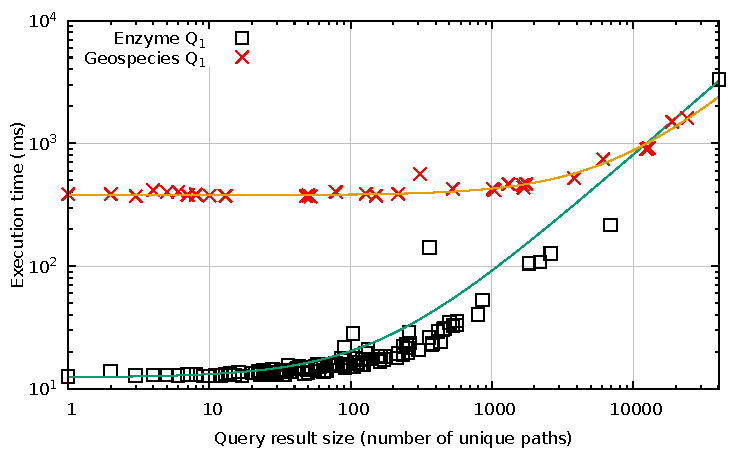
\includegraphics[width=0.5\textwidth]{data/time_per_paths_SCO.pdf}
    \caption{Execution time for $Q_1$ query}
    \label{fig:time_per_paths_SCO}
  \end{center}
\end{figure}


\begin{figure}[h]
  \begin{center}
    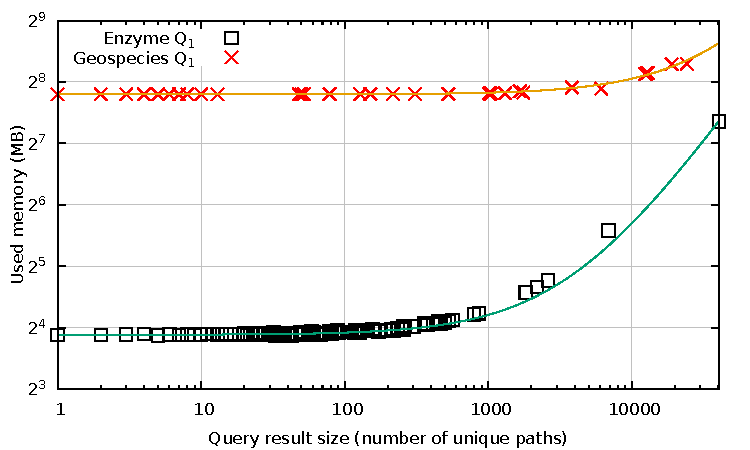
\includegraphics[width=0.5\textwidth]{data/mem_per_paths_SCO.pdf}
    \caption{Memory consumption for $Q_1$ query}
    \label{fig:mem_per_paths_SCO}
  \end{center}
\end{figure}


Time and memory measurements results for $Q_1$ query are provided in figures~\ref{fig:time_per_paths_SCO} and~\ref{fig:mem_per_paths_SCO} respectively.


\begin{figure}[h]
  \begin{center}
    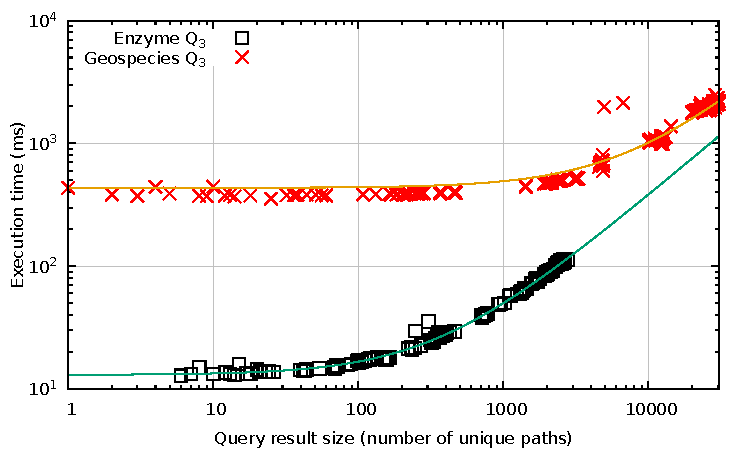
\includegraphics[width=0.5\textwidth]{data/time_per_paths_NT.pdf}
    \caption{Execution time for $Q_3$ query}
    \label{fig:time_per_paths_NT}
  \end{center}
\end{figure}

\begin{figure}[h]
  \begin{center}
    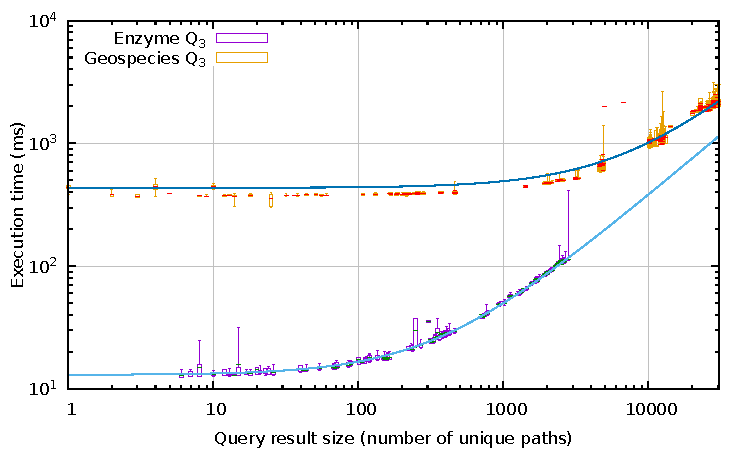
\includegraphics[width=0.5\textwidth]{data/time_per_paths_NT_boxplot.pdf}
    \caption{Execution time for $Q_3$ query (boxplot)}
    \label{fig:time_per_paths_NT_boxplot}
  \end{center}
\end{figure}


Time measuremet results for $Q_3$ query are provided in two ways: only average values for each query result size (figure~\ref{fig:time_per_paths_NT}) and standard boxplot to provide information about vales distribution (figure~\ref{fig:time_per_paths_NT_boxplot}). We can see that number of outliers is small. Note that the number of measurements for each query result size is different, so in some cases we have jus single points instead of boxes (it means that there is only one result of such size).


\begin{figure}[h]
  \begin{center}
    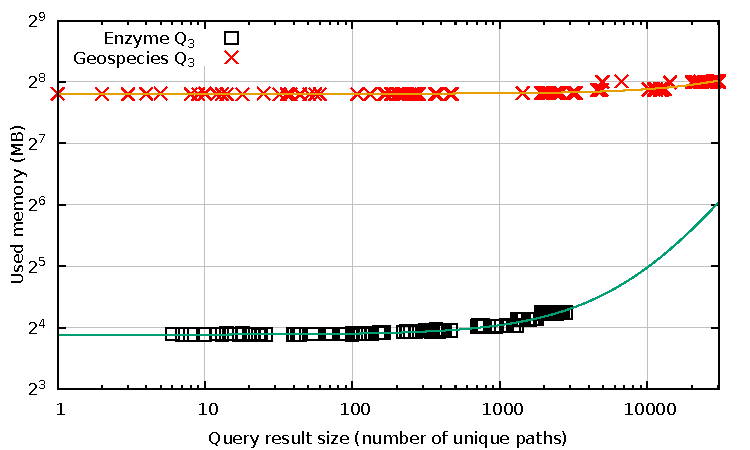
\includegraphics[width=0.5\textwidth]{data/mem_per_paths_NT.pdf}
    \caption{Memory consumption for $Q_3$ query}
    \label{fig:mem_per_paths_NT}
  \end{center}
\end{figure}

Memory consumption for $Q_3$ query is presented in figure~\ref{fig:mem_per_paths_NT}.

Also we can see, that for provided queries and graphs time and memory consumption are not depend on query: for similar result sizes reqired time and memory are similar for all qieryes.

\end{document}
